\documentclass{beamer}
\usepackage[T1]{fontenc} %svenska tecken, åäö egna bokstäver
\usepackage[utf8]{inputenc} %vald teckenkodning
\usepackage[swedish]{babel} %svensk dokumentstandard engelska rubriker
\usepackage{multicol}
\usetheme{Frankfurt}
\setbeamertemplate{navigation symbols}{}
\title[Mister Roboto]{Robotics Safety}
\author{Patrik, Niklas, Pär, Mattias, Olle, Benjamin}
\institute{Computer Vision}
\date{\today}
\graphicspath{{images/}}
\usepackage{algorithm2e}
\begin{document}

\begin{frame}{TSBB11 - CDIO Project}
	\titlepage
\end{frame}

% Robot
\begin{frame}{Robot and controller}
\begin{itemize}
\item Controller, (DX100)
\begin{itemize}
\item Controlls the robot (SIA20D)
\begin{itemize}
\item Via programming pendant
\end{itemize}
\item Receives robot orientation 
\end{itemize}
\end{itemize}

\begin{figure}[H]
	\begin{center}
	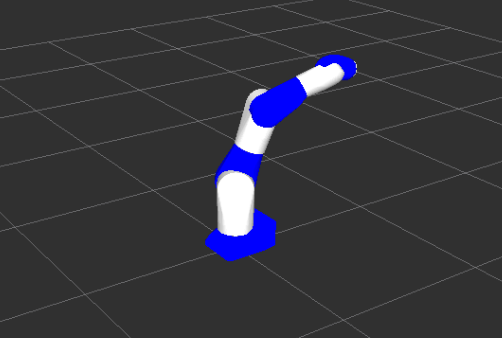
\includegraphics[scale = 0.05]{robot}
	\end{center}
	\end{figure}

\end{frame}
\begin{frame}{Controller - Computer interface}


\begin{itemize}
\item ROS (Robot Operating System)
\begin{itemize}
	\item OpenCV
	\item PCL (point cloud library)
\end{itemize}
\item Connected via ethernet
\item Joint states $[rad]$ to computer

\item ''Send'' motion commands to controller
\end{itemize}

\end{frame}



% Backgroundsegmentation

\begin{frame}{Background segmentation}

\begin{columns}
\column{0.5\textwidth}
	\begin{itemize}

	\item From OpenCV
	\begin{itemize}
	\item Gaussian mixtures
	\end{itemize}
	\item Applied to depth image
	\begin{itemize}
	\item Binary foreground
    \end{itemize}
	\end{itemize}
\column{0.5\textwidth}
	
	\begin{figure}[H]
	\begin{center}
	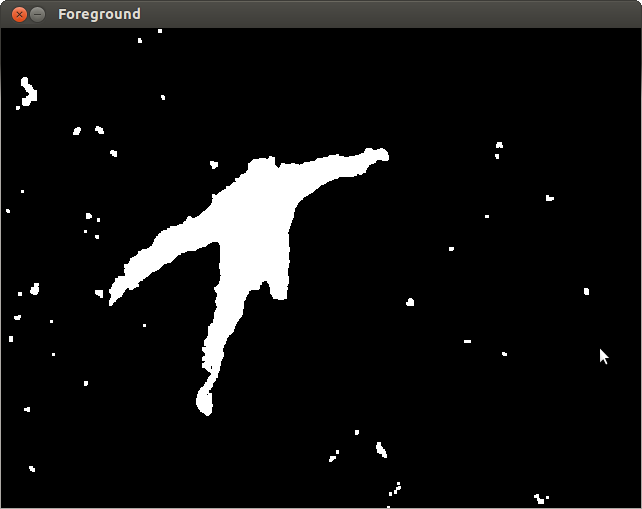
\includegraphics[width = 5cm]{foreground}
	\end{center}
	\end{figure}
	\end{columns}
\end{frame}
\begin{frame}{Background segmentation}

\begin{itemize}
	\item Method constructed for RGB, but
	\item Performance well on depth image
	\item Kinect uses a projection pattern
	\begin{itemize}
		\item Small influence of shadows
		\item Reflections give NaN values
	\end{itemize}
	\end{itemize}
\end{frame}
% PointCLoudCalc 

\begin{frame}{Calculation of Point Cloud}
	\begin{itemize}
	\item Known Values are:
	\begin{itemize}
	\item Depth value
	\item Pixel position 
	\end{itemize}
	\end{itemize}
\end{frame}

%Clustering of point cloud

\subsection{Clustering}
Clustering
The clustering node receives a point cloud from the background segmentation node corresponding to the extracted foreground i.e. moving objects. The purpose of the clustering node is to divide the entire point cloud into individual objects. It also removes noise and objects that are not considered to be large enough.  

The reason why individual objects are necessary is because the closest distance to every object compared to the robot is desired. It is not sufficient to know the distance from the closest point in the whole point cloud to the robot. Separating the entire point cloud into individual clouds also provides the possibility for an implementation of tracking point cloud objects. 

The separation of objects is done by separating the entire point cloud into clusters. This is done using an euclidean cluster extraction algorithm. A simple outline of the algorithm is that for each point, check whether there is another point within a given radius and if so assign this point to the same cluster. In other words, the points that are close enough are concatenated to each other. If there is no point within the given radius that already is assigned to a cluster then the point should correspond to a new cluster. The cluster extraction is based on the algorithm given by Point Cloud Library \cite{CE}.
% Calibration between coordinate systems.

\subsection{Calibration}
To relate the camera system to the world system defined by a fixed point in a calibration pattern the system has to be calibrated. For calibration of the camera intrinsic parameters and distortions from the pinhole camera model the system uses the models and methodology described by Zhang, 2000 \cite{zhang}. This is performed offline.

For online calibration of the camera extrinsics the same distortion and intrinsic parameters are used with a world fixed calibration pattern.

The online calibration is very computationally expensive however since the system is supposed to be stationary, recalibration is only done once a second to compensate for small adjustments on the system. The possibility for the camera to move still exists and if so the system would be maladjusted and give out wrong answers which is why the online calibration is performed.

Most of the building blocks of the calibration is implemented by the OpenCV library \cite{camcal}. 

\subsubsection{Intrinsic calibration}
Before image distortions the projection of the 3D-world to the image plane is described by this matrix:

\[\begin{bmatrix}
x \\
y \\
w
\end{bmatrix}
=
\begin{bmatrix}
 f_x & 0   & c_x \\ 
 0   & f_y & c_y \\ 
 0   & 0   & 1
\end{bmatrix}
\begin{bmatrix}
X \\
Y \\
Z
\end{bmatrix}\] 

Where $f_x$ and $f_y$ are the number of pixels per unit of length, $c_x$ and $c_y$ are the center pixel coordinates of the image. X, Y and Z are the camera relative positions of a visible point with x, y and w as the homogeneous representation of the pixel coordinate where the point is projected.

Distortions from this model is modelled as radial distortion as well as tangential distortions. Radial distortions produce a fish-eye effect on the image and is compensated for with this model:

\[x_{radialcorrected} = x\cdot (1+k_1\cdot r^2 + k_2\cdot r^4 + k_3\cdot r^6)\]
\[y_{radialcorrected} = y\cdot (1+k_1\cdot r^2 + k_2\cdot r^4 + k_3\cdot r^6)\]

Tangential distortions due to the lense not being perfectly aligned is compensated with this model:

\[x_{tangentialcorrected} = x + 2p_1xy+p_2(r^2+2x^2)\]
\[y_{tangentialcorrected} = x + p_1(r^2+2y^2)+2p_1xy\]

Since this is a standard model external libraries have support for these parameters and the error correction from calculating the distortion parameters will cascade into other functions. Intrinsic and distortion calibration is done offline and the parameters are saved into a YAML file.

\subsubsection{Extrinsic calibration}
To relate the position and state of the robot to the camera there needs to be a reference between a fixed robot frame and the camera frame. To solve this a calibration pattern is placed at a known position relative to the robot.

This calibration pattern is then detected in the image and the solution to the PnP (Perspective-n-Point) problem with the camera parameters is used as extrinsic parameters.

To minimize noise and increase robustness a large chessboard pattern with 6x8 known points is used for calibration. However there is no known analytical solutions to the PnP problem for n > 3 so the problem is solved using optimization (minimization of the sum of squared reprojection errors) with the Levenberg-Marquardt iterative optimization algorithm.

To prevent the optimization getting stuck on local optima the system uses initial solutions provided by the P3P solver.
The points used for these initial solution are the four corners of the chessboard, three to solve the P3P problem and one to validate which of the four possible solutions is consistent with the rest of the data.
The P3P solver used in OpenCV provides an unknown number of solutions since the algorithm does not handle all possible cases. 

The PnP solver then uses these initial solutions to find the optimal solution.
To verify that the provided solution is correct the system checks that the x-axis in the found coordinate system is flipped compared to the x-axis specified by the camera.
This is necessary due to the problem of unknown numbers of solutions from the P3P solver.


\subsubsection{tf}
The tf subsystem is a built in part of ROS for managing transformations between different coordinate systems. It is written and maintained by Tully Foote. The tf package takes the different transformations of the system as input. Using them it can then provide the position of a point in an arbitrary coordinate system at any point in time.

\subsubsection{Transformation of robot joints}
Since information regarding the design of the robot is provided the transformations between the joints can be obtained. The tf package then makes it possible to transform the robot and its joints into a given coordinate system.

\subsubsection{Transformation into camera coordinate system}
A static transformation between calibration pattern and the base of the robot in world coordinates is set. Given the transformation from camera to calibration pattern, it is possible to transform each joint to the camera coordinate system. This results in a set of joints on which the distance calculation to moving objects in the scene can be performed. 

% Distance Calculation 

\begin{frame}{Calculation of Distances}
	Distances between objects and robot	
	\begin{algorithm}[H]
 %\SetLine % For v3.9
 \SetAlgoLined % For previous releases [?]
 \KwData{Robot Joints, Clusters}
 \For{Every point in a cluster}{
        \For{Every Joint position}{
        Check distance between Joint and cluster point\;
  \If{distance < minDistance}{
  distance = minDistance;
 }
 }
 }
 \caption{Distance Calculation}
\end{algorithm}
\end{frame}


% Tracking of Objects

\subsection{Tracking}
The system uses a background segmentation which has a learning rate. This means that the system  adapts its considered background during runtime. Since the system is adaptive, people who are standing still will disappear after a while. For that situation the system is not safe. This problem is solved by tracking objects found in the scene. 

%The tracking algorithm will save information of objects that disappears in the scene and the %robot will not continue working in normal pace until the object has left the safety zone. The %system is not required to keep track of objects that is occluded and objects that interfere %with each other. Since the requirement of the tracker is rather low the implementation is %simple and has no guarantees of actually tracking objects throughout the entire scene if %occlusion occurs.

To keep track of all objects in the scene an object list is used to contain information about all objects. The information describes for all objects the relationship to the robot, the mean point of the cluster and if it is visible or not. 

%and an index towards the object which is closest to the robot. Every object contains the %closest joint on the robot, closest point on the object and the distance between them, which 
%is called the min-distance. It will also contain an average point and a bool-variable which %tells if the object is visible or not.  

Every cluster which is classified as an object will then correspond to an object in the object list. When an object is calculated in a new frame its average point will be compared to the average points of the objects in the object list. If there are any objects in the object list which does not correspond to any objects in the current frame there are theoretically two different possibilities, the object has moved out of the camera view or the object has blended into the background. To know which one it is the min-distance of the object is used. If the distance is sufficiently large it is assumed that the object has moved out of the camera view and the object will then be removed from the object list. If the distance is sufficiently small the object is assumed to have blended into the background, the object will then be kept in the object list but it will be marked as not visible. Objects that are outside the safety zones will not be tracked. Since new objects can not occur inside the safety zones another advantage with the tracking is that it will reduce noise.

\begin{figure}[H]
\begin{center}
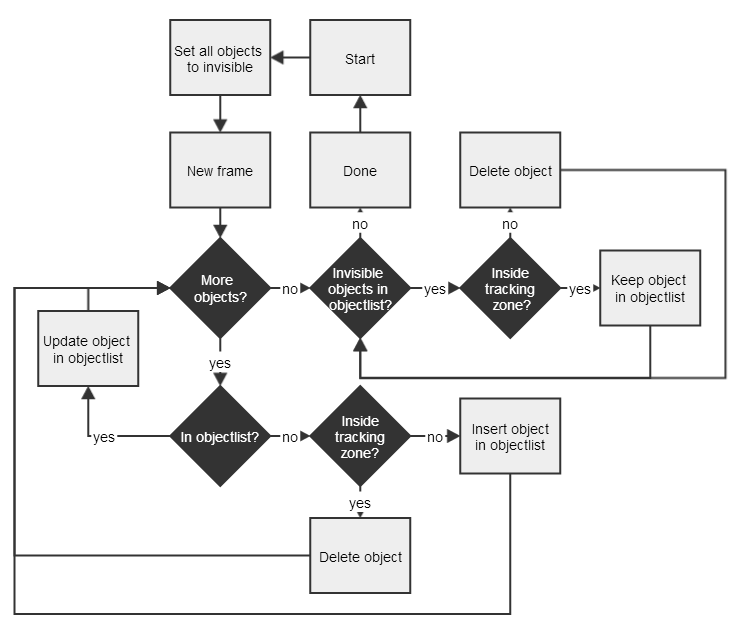
\includegraphics[width=12 cm]{tracking}
\caption{Flowchart of tracking algorithm}
\label{tracking}
\end{center}
\end{figure}

\subsection{Visualization}

The results of the system is visualized in RViz, which is a 3D visualization tool for ROS. 

\subsubsection{Robot}
The data received from the controller are the joint states.
The visualizer, RViz, uses these states when determining the robots pose.
The robots construction is predefined and RViz only requires the joint states to draw the robot.
The length between the nodes and its appearance was provided by developer, in mesh format.
 
\begin{figure}[H]
\begin{center}
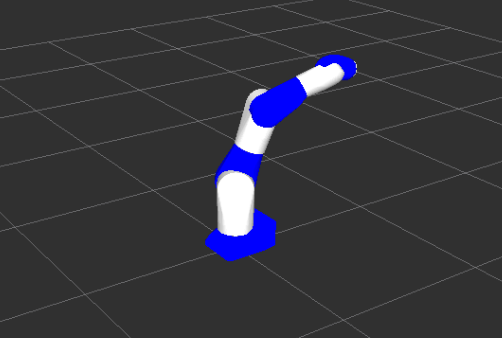
\includegraphics[width=12 cm]{robot}
\caption{3D-model of robot.}

\end{center}
\end{figure}

\subsubsection{Objects}
The objects in the image that the tracking algorithm considers being real moving objects are visualized. They are published as point clouds so that Rviz can subscribe to them and visualize them. If the tracking algorithm believes that an object has disappeared because of non-movement, it keeps the last seen point cloud of the object i.e. static objects in the scene are objects that the system thinks are standing still. 

\begin{figure}[H]
\begin{center}
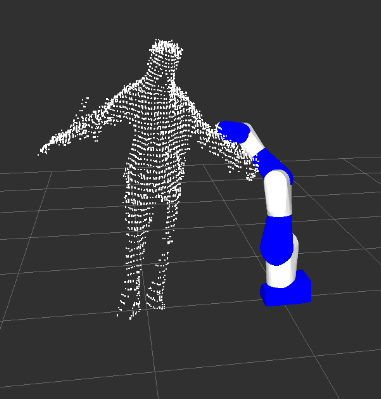
\includegraphics[width=12 cm]{humanandrobot}
\caption{Clustered object beside the robot.}

\end{center}
\end{figure}


\subsubsection{Distances}
To visualize the resulting state of the system (the current safety zone) a line between the closest object and the closest joint of the robot is drawn. This line switches color depending on which state the system is in. The color of the line is thereby the result of the system. 

\begin{itemize}
  \item Red - Emergency zone
  \item Yellow - Safety zone 1 
  \item Green - Safety zone 2
  \item No line - Outside safety zone 2 
\end{itemize}

\begin{figure}[H]
\begin{center}
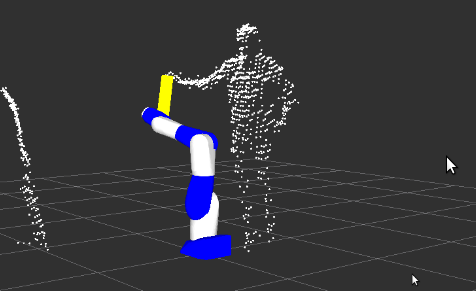
\includegraphics[width=12 cm]{resultat1}

\caption{Result}
\end{center}
\end{figure}

\begin{figure}[H]
\begin{center}
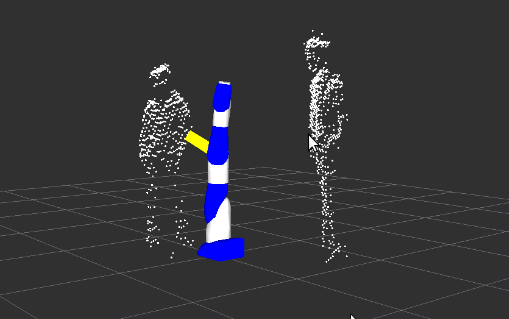
\includegraphics[width=12 cm]{resultat2}

\caption{Result}
\end{center}
\end{figure}

% Results 

\begin{frame}{Results}

Good
	\begin{itemize}
	\item Great performance with one object
	\item Background subtraction is reliable for moving objects
	\end{itemize}
	
	\vspace{4mm}
Slightly less Good
	\begin{itemize}
	\item Background subtraction is less reliable for detecting relevant objects
	\item Performance issues
	\end{itemize}
	
\end{frame}

\begin{frame}
	\Huge
	\centering
	\textbf{Questions?}
\end{frame}
 
\end{document}